\newpage
	\section{W} \label{sec:W}
		\subsection{WALKTHROUGH} \index{Walkthrough} \label{walkthrough} %7 dicembre - Verifica e validazione
		Tecnica che consiste nel cercare la presenza di difetti in ogni dove, non sapendo dove. È un metodo di lettura pratico come \underline{\hyperref[inspection]{Inspection}} la cui efficacia dipende dall'esperienza dei verificatori. La strategia, per il codice, prevede il percorrerlo tutto simulandone possibili esecuzioni. \\
		Le sue attività sono divise in 4 e in ognuna svolta deve essere fatta la documentazione:
		\begin{itemize}
			\item fase 1: pianificazione;
			\item fase 2: lettura;
			\item fase 3: discussione;
			\item fase 4: correzione dei difetti;
		\end{itemize}
		
		\subsection{WORK BREAKDOWN STRUCTURE} \index{WBS} \label{wbs}
		È una struttura gerarchica di attività che si compongono di sotto-attività non necessariamente sequenziali e univocamente identificate. 
		%A work-breakdown structure (WBS) in project management and systems engineering, is a deliverable-oriented breakdown of a project into smaller components. A work breakdown structure is a key project deliverable that organizes the team's work into manageable sections.
		
		\begin{figure}[H]
			\centering
			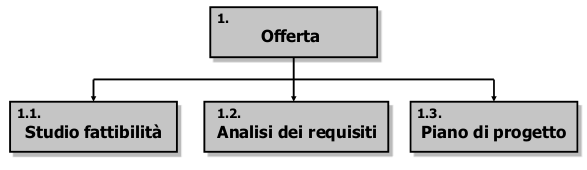
\includegraphics[width=0.8\textwidth]{img/wbs}		
			\caption{Esempio di diagramma di WBS.}
		\end{figure} 
	
	
